\documentclass{article}

\usepackage{ucs}

\usepackage[utf8x]{inputenc}
\usepackage[greek, english]{babel}
\usepackage{alphabeta}
\usepackage{lmodern}

\usepackage[linguistics]{forest}

\usepackage{listings}

\usepackage{graphicx}
\graphicspath{./images/}

\usepackage{forest}

\title{Πρώτο μέρος εργαστηριακής εργασίας στο μάθημα Τεχνήτη Νοημοσύνη}
\date{2020-11-22}
\author{Ιάκωβος Μαστρογιαννόπουλος - cse242017102}

\definecolor{codegreen}{rgb}{0,0.6,0}
\definecolor{codegray}{rgb}{0.5,0.5,0.5}
\definecolor{codepurple}{rgb}{0.58,0,0.82}
\definecolor{backcolour}{rgb}{0.95,0.95,0.95}

\lstdefinestyle{mystyle} {
    backgroundcolor=\color{backcolour},
    commentstyle=\color{codegreen},
    keywordstyle=\color{magenta},
    numberstyle=\tiny\color{codegray},
    stringstyle=\color{codepurple},
    basicstyle=\ttfamily\footnotesize,
    breakatwhitespace=false,
    breaklines=true,
    captionpos=b,
    keepspaces=true,
    numbers=left,
    numbersep=5pt,
    showspaces=false,
    showstringspaces=false,
    showtabs=false,
    tabsize=2
}

\lstset{style=mystyle}

\begin{document}
    \pagenumbering{gobble}
    \maketitle
    
    \newpage
    \tableofcontents
    \newpage
    \lstlistoflistings

    \newpage
    \pagenumbering{arabic}
    \section{Πρόλογος}

    \paragraph{}
    Στη συγκεκρίμενη εργασία του μαθήματος <<Τεχνητής Νοημοσύνης>> είχαμε να μελετήσουμε το προβλήμα του parking. Βέβαια,
    για να μπορέσουμε να φτάσουμε στο σημείο της υλοποίησης του κωδικά, πρώτα πρέπει να εξηγηθούν μερικά πραγμάτα με το ποιο είναι
    το πρόβλημα, πώς μπορούμε να το υλοποιήσουμε και ποια θα είναι τα πιθανά αποτελέσματα που θα μπορούσαμε να πάρουμε πίσω.  
    Όπως έχει αναφερθεί και σε email, την εργασία την κάνει ένα ατόμο μόνο του. Η γλώσσα προγραμματισμού που υλοποιήθηκαν οι αλγόριθμοι
    είναι η Python, στον IDE Pycharm και συγκεκριμένα ήταν η έκδοση 3.8.6.

    \newpage
    \section{Κατανόηση προβλήματος - Προβλήμα του Parking}
    \paragraph{}
    Το πρόβλημα που έχουμε να λύσουμε είναι το πρόβλημα του Parking. Θεωρετηκά, υπάρχει ένας αυτόματος οδηγός ο οποίος προσπαθεί να βρει
    ελευθέρο χώρο για να γεμίσει τα αμάξια που θέλουν να μπουν μέσα στο Parking. Υπάρχουν Ν spaces από τα οποία θα μπορούσαν μερικά από αυτά
    να ήταν τελείως άδεια, ενώ κάποια αλλά να είχαν μια πλατφόρμα.

    \paragraph{}
    Σκοπός είναι να βρίσκει τις πλατφόρμες και από εκεί να καταλαβαίνει ποιες από αυτές έχουν ελεύθερο χρόνο και να τις γεμίζει. Τα βήματα που
    πρέπει να ακολουθήσουμε είναι τα εξής:

    \begin{itemize}
        \item Να βρίσκει σε ποιο node με πλατφόρμα υπάρχει ελεύθερη θέση
        \item Να τρέχει έναν αλγόριθμο αναζήτησης και να βρίσκει το πιο γρήγορο path
        \item Να ανταλλάζει θέση τα nodes μεταξύ τους, έτσι ώστε το node με την άδεια πλατφόρμα να πηγαίνει στην θέση 1
        \item Τέλος να έχει κάποιον στόχο που όταν τον εκπληρώσει να λήγει το πρόγραμμα
    \end{itemize}

    \newpage
    \section{Μοντελοποίηση του προβλήματος}
    \subsection{Χώρος καταστάσεων}
    \paragraph{}
    Χώρο καταστάσεων ενός προβλήματος ονομάζουμε το σύνολο των πιθανών καταστάσεων, στις οποίες μπορούν να βρεθούν οι καταστάσεις του προβλήματος.
    Στο πρόβλημα του parking τα αντικείμενα είναι τα αυτοκίνητα, τα spaces και οι πλατφόρμες. Μια κατάσταση είναι εάν το space έχει πλατφόρμα ή εάν η
    πλατφόρμα έχει ελεύθερο χώρο για να χωρέσει αυτοκίνητα.

    \subsection{Αρχική κατάσταση}
    \paragraph{}
    Η αρχική κατάσταση του Parking απαιτεί να υπάρχουν 4 spaces, όπου μόνο 3 από αυτά έχουν ελεύθερες θέσεις, και 3 αυτοκίνητα που περιμένουν απέξω για 
    να μπουν μέσα. Στην προέκταση, μας ζητήθηκε να αυξήσουμε τον αριθμό των spaces.

    \subsection{Τελική κατάσταση}
    \paragraph{}
    Δεν υπάρχει κάποια συγκεκριμένη τελική κατάσταση για το συγκεκριμένο πρόβλημα. Ομώς, εμείς μπορούμε να θεωρήσουμε ως τελική κατάσταση όταν όλες οι πλατφόρμες
    έχουν γεμίσει με αυτοκίνητα.

    \subsection{Τελεστές προβλήματος}
    \paragraph{}
    Στο πρόβλημα μας έχουμε δύο τελεστές:

    \begin{itemize}
        \item Τελεστή IN: ο Τελεστής όπου βάζει τα αυτοκίνητα μέσα στις πλατφόρμες.
        \item Tελεστή Neighbour: ο Τελεστής όπου διαβάζει τους γειτονές του κάθε node.
    \end{itemize}

    Στην κωδικοποίηση, βέβαια, η υλοποιήση των τελεστών ήταν λίγο διαφορετική, αλλά η ίδεα παραμένει ίδια.

    \newpage
    \section{Κωδικοποίηση}
    \subsection{Ορισμός κατάστασης}
    \paragraph{}
    Για την κωδικοποιήση του προβλήματος, φτιάξαμε 2 dictionaries όπου στο ένα έχουμε αποθηκευμένο τις γειτονικές σχεσείς των nodes, ενώ στο αλλό την κατάσταστη του κάθε
    node (πχ εάν έχει πλατφόρμα ή εάν είναι άδειο).

    \paragraph{}
    Δηλαδή, η αρχική μας κατάσταση θα είναι η εξής:

    \begin{lstlisting}[language=Python]
        neighbours = {
            '1': set(['2', '4']),
            '2': set(['1', '3']),
            '3': set(['2', '4', '6']),
            '4': set(['1', '3', '5']),
            '5': set(['4', '6']),
            '6': set(['3', '5'])
        }

        spaces = {
            '1': ["Empty", "NO"],
            '2': ["Platform 1", "NO"],
            '3': ["Platform 2", "NO"],
            '4': ["Platform 3", "NO"],
            '5': ["Platform 4", "NO"],
            '6': ["Platform 5", "NO"]
        }
    \end{lstlisting}

    Ως τελική κατάσταση, μπορούμε να ορίσουμε ότι όλα τα spaces είναι γεμάτα. 

    \begin{lstlisting}[language=Python]
        spaces = {
            '1': ["Empty", "NO"],
            '2': ["Platform 1", "YES"],
            '3': ["Platform 2", "YES"],
            '4': ["Platform 3", "YES"],
            '5': ["Platform 4", "YES"],
            '6': ["Platform 5", "YES"]
        }
    \end{lstlisting}

    \newpage
    \subsection{Κωδικοποιήμενοι Τελεστές Ελέγχου}
    \paragraph{}
    Έχουμε δύο τελεστές ελεγχού

    \begin{center}
        \begin{tabular}{|c|c|}
            \hline
            Τελεστής ελέγχου & Λειτουργία \\
            \hline
            is empty & Ψαχνεί να βρει σε ποιο node έχει αδεία πλατφόρμα. \\
            \hline
            is goal & Κοιτάει κάθε στοιχείο του γράφου εάν η καταστάση του είναι ίδια με του goal state. \\
            \hline
        \end{tabular}
    \end{center}

    Ακολουθεί αναλυτικά το πως δουλευουν αναλυτικά

    \subsection{is empty}

    \lstinputlisting[language=Python, caption=Is Empty Algorithm]{../Parking/is_empty.py}

    \paragraph{}
    Μπορούμε να παρατηρήσουμε ότι κοιτάει τρία πραγμάτα:

    \begin{itemize}
        \item Εάν το space που είμαστε τώρα δεν είναι empty
        \item Εάν το space που είμαστε τώρα έχει πλατφόρμα και είναι άδεια
        \item Εάν το goal της πλατφόρμα που έχει το space, την θέλουμε άδεια.
    \end{itemize}

    \paragraph{}
    Τα αποτελέσματα από το test που έχω γράψει μας επιστρέφουν το εξής:

    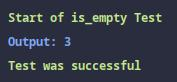
\includegraphics{images/is_empty.jpeg}

    \paragraph{}
    Μπορούμε να παρατηρήσουμε ότι βρήκε σωστά ότι στο 3ο index έχει άδεια θέση.

    \subsection{is goal}

    \lstinputlisting[language=Python, caption=Is Goal Algorithm]{../Parking/is_goal.py}

    \paragraph{}
    Εδώ παρατηρούμε ότι ο αλγόριθμος κοιτάει όλα τα nodes του state, και τα συγκρίνει με τα ίδια nodes του goal state έαν
    έχουν την ίδια τιμή. Εάν βρει ένα ζευγάρι που δεν έχει την ίδια τιμή, επιστρέφει False, ενώ εάν ολοκληρωθεί το loop και δεν βρει
    κάτι, σημαίνει ότι έχει βρεθεί το goal και επιστρέφει True. 

    \paragraph{}
    Πάμε να δούμε τα αποτελέσματα του test που έχει γραφτεί:

    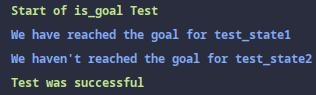
\includegraphics{images/is_goal.jpeg}

    \paragraph{}
    Για το πρώτο test state, μπορούμε να δούμε ότι βρήκε ότι έχει ολοκληρωθεί και εκπληρώσει τον σκοπό του, ενώ για το δεύτερο δεν τον έχει εκπληρώσει.

    \subsection{Τελεστές Μετάβασης}
    Η κωδικοποιήση δυστυχώς δεν έχει ξεχωρίστους τελεστές μετάβασης, όλα βρίσκονται μέσα στο find solution, λόγω ελείψης χρόνου. Όποτε πάμε να δούμε αναλυτικά τι κάνει.

    \newpage
    \subsection{find solution}

    \lstinputlisting[language=Python, caption=Find Solution Algorithm]{../Parking/find_solution.py}
    \paragraph{}
    Μπορούμε να δούμε ότι το πρώτο πράγμα που κάνει είναι να βρει σε ποιο index βρίσκεται η άδεια πλατφόρμα με την χρήση του is empty που μελετήσαμε προηγουμένος.
    Μετά, τρέχει τον αλγόριθμο αναζήτησης που έχουμε επιλέξει να τρέξει για να πάρουμε πίσω έναν πίνακα που έχει μέσα το Front της μεθόδου, όπου μετά τον τρέχουμε στην
    συνάρτηση min με key το len για να βρούμε το γρηγορότερο path. Πιο αναλυτικά για το πως δουλεύει κάθε αλγόριθμος αναζήτησης θα το δούμε στο επόμενο κεφάλαιο. Στην συνέχεια
    τρέχει την swap. Παμέ να δούμε και τον αλγόριθμο swap.
    
    \newpage
    \lstinputlisting[language=Python, caption=Swap Algorithm]{../Parking/swap.py}
    \paragraph{}
    Η swap είναι μία βοηθητική συνάρτηση μετάβασης που την λίστα από τον αλγόριθμο αναζήτησης και ανταλλάζει τα στοιχεία μεταξύ τους επιστρέφοντας πίσω μία νέα λίστα.

    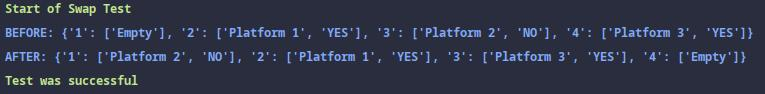
\includegraphics[scale=0.7]{images/swap.jpeg}
    \paragraph{}
    Στην συνέχεια, το find solution αλλάζει την τιμή στην θέση 1, αφού εκεί θέλουμε να γινόνται όλες οι αλλάγες και το κάνει YES, ότι είναι γεμάτο, και επιστρέφει πίσω
    ένα τελικό αποτέλεσμα. Παμέ να δούμε τα αποτελέσματα του find solution.

    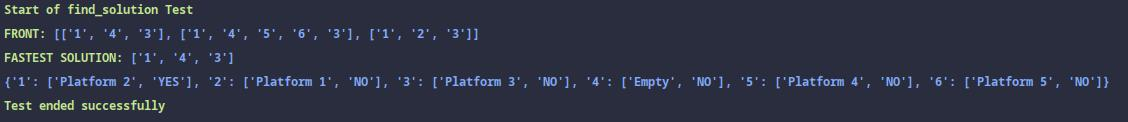
\includegraphics[scale=0.5]{images/find_solution.jpeg}
    \paragraph{}
    Μπορούμε να δούμε ότι βρίσκει ένα Front από τον αλγόριθμο αναζήτησης (σε αυτή την περιπτώση ήταν ο DFS) και επιτυχημένα βρίσκει το πιο γρήγορο μονοπάτι, κάνει το swap
    και παίρνει σωστά αποτελέσματα

    \newpage
    \section{Αλγόριθμοι Αναζήτησης}
    Οι αλγόριθμοι αναζήτησης που υποστιρίζει η κωδικοποιήση μας είναι τρεις:
    
    \begin{itemize}
        \item Ο Αλγόριθμος DFS
        \item Ο Αλγόριθμος BFS
        \item Ο Αλγόριθμος BestFS
    \end{itemize}

    \paragraph{}
    Στην συνέχεια θα δούμε αναλυτικά πως δουλεύει ο καθένας του ξεχωριστά.

    \subsection{DFS}
    \lstinputlisting[language=Python, caption=DFS Algorithm]{../Parking/DFS.py}

    \paragraph{}
    O αλγορίθμος βασίζετε στην αναδρομική διαδικάσια η οποία δέχεται σαν είσοδο μία κορυφή u και επισκέπτεται αναδρομικά το αριστερό και μετά το δεξίο του γειτονική κορυφή. 
    Στην πραγματικότητα βεβαία υλοποιεί μία στοίβα, με ιεραρχία LIFO. Στο συγκεκριμένο παράδειγμα, έχουμε μια παραλλαγή του DFS όπου παρακολούθει παραλλήλα κάθε πιθανή πορεία
    που θα μπορούσε να πάρει το node για να φτάσει στον σκοπό του. Στον κώδικα του DFS παρατηρούμε ότι δεν επιστρέφει πίσω μεταβλήτες. Στην πραγματικότητα, επιστρέφει 
    πίσω generators τιμών και ετσί μειώνεται η πολυπλοκότητα του αλγοριθμού, αφού δεν χρειάζεται να αποθηκεύει την ίδια λίστα ξανά και ξανά. 

    \paragraph{}
    Παμέ να δούμε θεωρετικά το γράφο που χρησιμοποιούμε στο test case. Από το 1 εώς το 5, θα μας επιστρέψει το εξής tree:

    \begin{forest}
        [1
        [2
        [4
        [5]
        ][5]]]
    \end{forest}

    \paragraph{}
    Όποτε, εάν ο αλγόριθμος είναι σωστός πρέπει να δούμε το εξής αποτέλεσμα: [[1,2,4,5],[1,2,5]]. Ας τον τρέξουμε τον αλγόριθμο.

    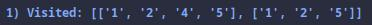
\includegraphics{images/DFS.jpeg}

    \paragraph{}
    Βλεπούμε ότι όντως παίρνουμε το σωστό αποτέλεσμα, όποτε είναι σωστή η υλοποιήση του DFS.

    \newpage
    \subsection{BFS}
    \lstinputlisting[language=Python, caption=BFS Algorithm]{../Parking/BFS.py}

    \paragraph{}
    Η διάσχιση κατά πλάτος (BFS) πρώτα επισκέπτεται όλους τους κόμβους που βρίσκονται στο ίδιο επείπεδο και μέτα προχωράει στους επόμενους κόμβους. Με άλλα λόγια, αντί να υλοποιείται LIFO,
    έχουμε FIFO. Αλλή μια διάφορα μεταξύ DFS και BFS είναι ότι ο BFS δεν είναι αναδρομίκος. Όπως στον DFS, έτσι και στον BFS έχουμε μία παραλλαγή του αλγοριθμού όπου παρακολοθεί παράλληλα
    κάθε πιθανή πορία που θα μπορούσαμε να παρούμε.

    \newpage
    \paragraph{}
    Πάμε να δούμε το ίδιο πάραδειγμα που είχαμε δει στον BFS:

    \begin{forest}
        [1
        [2
        [5]
        [4
        [5]]]]
    \end{forest}

    \paragraph{}
    Οπότε εάν τρέξουμε τον κώδικα, περιμένουμε να δούμε το εξής αποτέλεσμα: [[1,2,5],[1,2,4,5]]. Ας τρέξουμε και τον αλγόριθμο.

    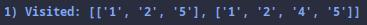
\includegraphics{images/BFS.jpeg}

    \paragraph{}
    Τα αποτελέσματα για άλλη μια φορά συμφωνούν μαζί μας, όποτε είναι σωστή και αυτή η υλοποιήση.

    \newpage
    \subsection{BestFS}
    \lstinputlisting[language=Python, caption=BestFS Algorithm]{../Parking/BestFS.py}

    \newpage
    \paragraph{}
    O BestFS είναι μια παραλλαγή του BFS. Βεβαία, πιστεύω ότι η υλοποιήση που έφτιαξα ότι δεν είναι σωστή και θα μπορούσε να βελτιωθεί. Περιμένουμε να δούμε ένα παρόμοιο tree, 
    με αυτό του BFS, δηλαδή:

    \begin{forest}
        [1
        [2
        [5]
        [4
        [5]]]]
    \end{forest}

    \paragraph{}
    Οπότε εάν τρέξουμε τον κώδικα, περιμένουμε να δούμε το εξής αποτέλεσμα: [[1,2,5],[1,2,4,5]]. Ας τρέξουμε και τον αλγόριθμο.

    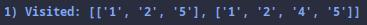
\includegraphics{images/BFS.jpeg}

    \paragraph{}
    Παρόλο που πήραμε ότι περιμέναμε, ακόμα δεν περιμένω να είναι σωστή η υλοποιήση.

    \newpage
    \section{Ενδεικτικά Τρεξίματα}
    \lstinputlisting[language=Python]{../main.py}

    \paragraph{}
    Αυτή είναι η main του προγράμματος. Πάμε να δούμε την εκτέλεση του με DFS, BFS και ΒestFS.

    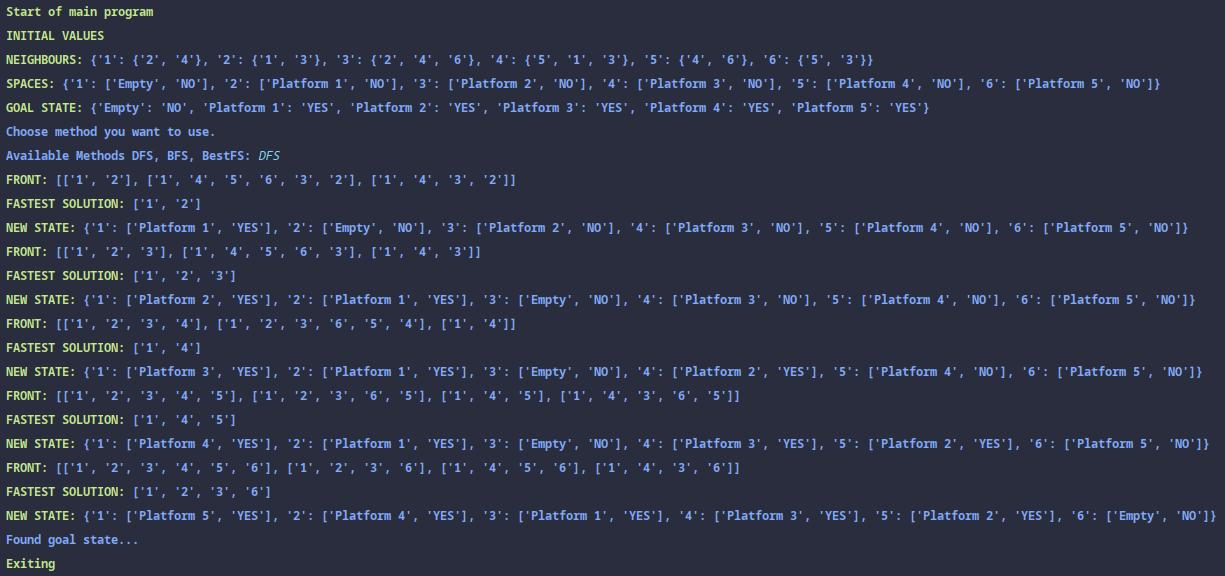
\includegraphics[scale=0.5]{images/main_dfs.jpeg}

    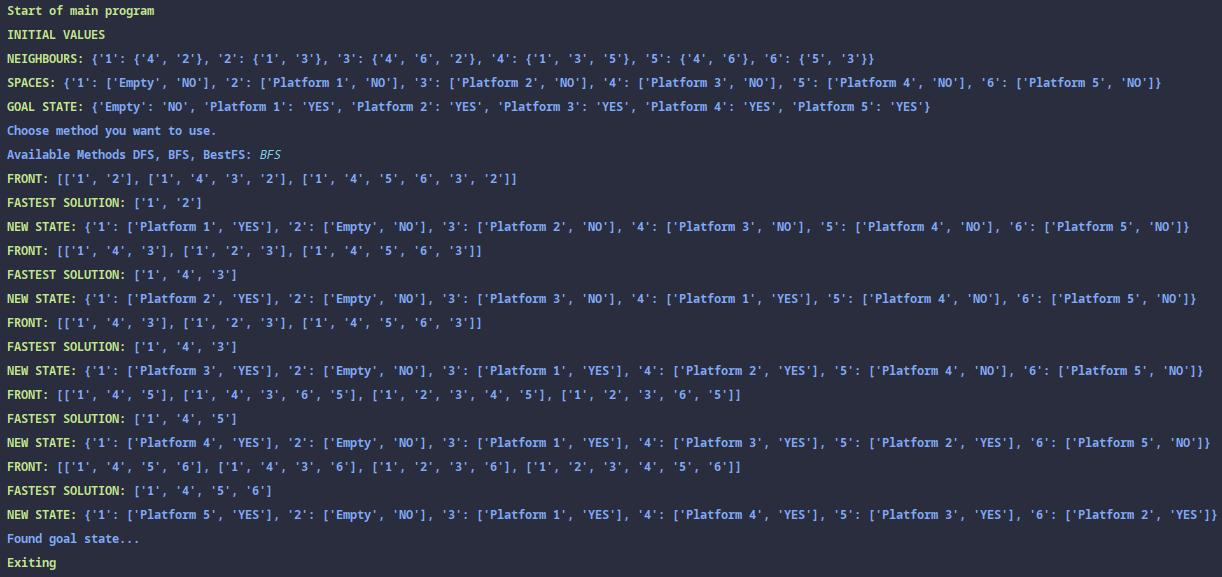
\includegraphics[scale=0.5]{images/main_bfs.jpeg}

    \newpage
    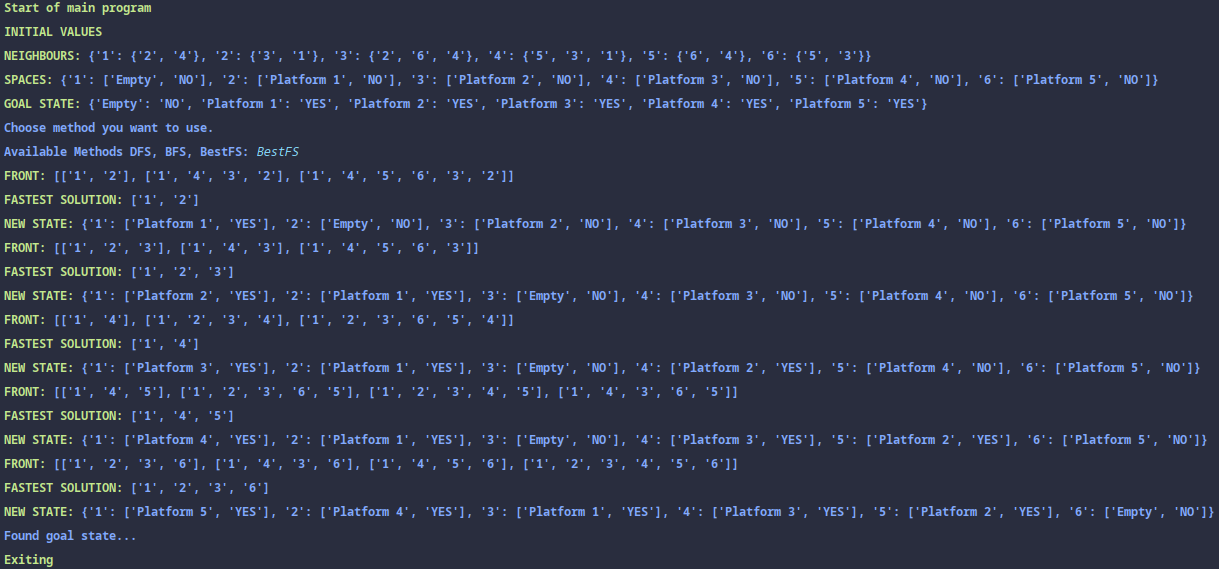
\includegraphics[scale=0.5]{images/main_bestFS.png}

    \section{Συμπεράσματα - Βελτιώσεις}
    \paragraph{}
    Μπορούμε να παρατηρήσουμε ότι ο BFS είναι πιο αποδοτικός απο τον DFS, αλλά ο DFS είναι πιο γρήγορος. Εάν υπήρχε σωστή υλοποιήση του BestFS, βεβαία, αυτός θα ήταν πιο γρήγορος.
    Μια βελτιώση που θα ήθελα να κάνω στην εργασία είναι η προσθήκη του Find Children, όμως δεν βρήκα κάποια χρησιμότητα στον τρόπο προσέγγισης που ακολούθησα ο ίδιος. Κατά τα αλλά,
    είδα μία πιο πρακτική χρήση των αλγορίθμων που έμαθα στους Αλγοριθμούς και Πολυπλοκότητα.

\end{document}